
%%%%%%%%%%%%%%%%%%%%%%%%%%%%%%%%%%%%%%%%%%%%%%%%%%%%%%%%%%%%%%%%%%%%%%%%%%%%%%
%%% 				Customizações do abnTeX2 para o IFCE    			   %%%
%%% 		Instituto Federal de Educação, Ciência e Tecnologia do Ceará   %%%
%%%																	       %%%
%%% Template disponível em: https://github.com/clodomirneto/IFCETeX2	   %%%
%%% Desenvolvedores do IFCETeX2: Professor Clodomir Silva Lima Neto	       %%%
%%% 							 Professor Marcelo Araújo Lima		       %%%
%%% 					  	     Professor Antonio Sergio de Sousa Vieira  %%%
%%% E-mails para contato: clodomir.neto@ifce.edu.br						   %%%
%%% 					  marcelo.alima@ifce.edu.br					       %%%
%%% 					  sergio.vieira@ifce.edu.br					       %%%
%%%																		   %%%
%%% Agradecimento: Thiago Nascimento 									   %%%
%%% https://github.com/thiagodnf/uecetex2                                  %%%
%%%%%%%%%%%%%%%%%%%%%%%%%%%%%%%%%%%%%%%%%%%%%%%%%%%%%%%%%%%%%%%%%%%%%%%%%%%%%%

%%%%%%%%%%%%%%%%%%%%%%%%%%%%%%%%%%%%%%%%%%%%%%%%%%%%%%%%%%%%%%%%%%%%%%%%%%%%%%
%%% 			Instruções para Uso do Template IFCETeX2	  			   %%%
%%%																	       %%%
%%% 1. Criar uma conta no Overleaf.									       %%%
%%% 2. No Ambiente Overleaf, clicar em Menu (canto superior esquerdo) 	   %%% 
%%% 3. Clicar em "Copiar Projeto".  									   %%%
%%% 4. Dê um novo nome para o Projeto. 								       %%%
%%%%%%%%%%%%%%%%%%%%%%%%%%%%%%%%%%%%%%%%% %%%%%%%%%%%%%%%%%%%%%%%%%%%%%%%%%%%%%

%%%%%%%%%%%%%%%%%%%%%%%%%%%%%%%%%%%%%%%%%%%%%%%%%%%%%%%%%%%%%%%%%%%%%%%%%%%%
%%% 				Customizações do abnTeX2 para o IFCE    			 %%%
%%% 		Instituto Federal de Educação, Ciência e Tecnologia do Ceará %%%
%%%																		 %%%
%%% Template disponível em: https://github.com/clodomirneto/IFCETeX2	 %%%
%%% Desenvolvedores do IFCETeX2: Professor Clodomir Silva Lima Neto		 %%%
%%% 							 Professor Marcelo Araújo Lima			 %%%
%%% E-mails para contato: clodomir.neto@ifce.edu.br						 %%%
%%% 					  marcelo.alima@ifce.edu.br						 %%%
%%%																		 %%%
%%% Agradecimento: Thiago Nascimento 									 %%%
%%% https://github.com/thiagodnf/uecetex2                                %%%
%%%%%%%%%%%%%%%%%%%%%%%%%%%%%%%%%%%%%%%%%%%%%%%%%%%%%%%%%%%%%%%%%%%%%%%%%%%%

%%%%%%%%%%%%%%%%%%%%%%%%%%%%%%%%%%%%%%%%%%%%%%%%%%%%%%%%%%%%%%%%%%%%%%%%%%%%
%%% 						Sequência do GitHub							 %%%
%%%																	     %%%
%%% git status + git add . + git commit + git push					     %%%
%%%%%%%%%%%%%%%%%%%%%%%%%%%%%%%%%%%%%%%%%%%%%%%%%%%%%%%%%%%%%%%%%%%%%%%%%%%%

\documentclass[
    a4paper,          % Tamanho da folha A4
    12pt,             % Tamanho da fonte 12pt
    chapter=TITLE,    % Todos os capitulos devem ter caixa alta
    %section=TITLE,   % Todas as secoes devem ter caixa alta
    oneside,          % Usada para impressao em apenas uma face do papel
    english,          % Hifenizacoes em ingles
    spanish,          % Hifenizacoes em espanhol
    brazil            % Ultimo idioma eh o idioma padrao do documento
]{abntex2}

% Importações de pacotes

\usepackage[utf8]{inputenc}                         % Acentuação direta
\usepackage[T1]{fontenc}                            % Codificação da fonte em 8 bits
\usepackage{graphicx}                               % Inserir figuras
\usepackage{amsfonts,amssymb,amsmath}               % Fonte e símbolos matemáticos
\usepackage{booktabs}                               % Comandos para tabelas
\usepackage{verbatim}                               % Texto é interpretado como escrito no documento
\usepackage{multirow,array}                         % Múltiplas linhas e colunas em tabelas
\usepackage{indentfirst}                            % Endenta o primeiro parágrafo de cada seção.
\usepackage{listings}                               % Utilizar codigo fonte no documento
\usepackage[table]{xcolor}% http://ctan.org/pkg/xcolor
\usepackage{microtype}                              % Para melhorias de justificação?
\usepackage[portuguese,ruled,lined]{algorithm2e}    % Escrever algoritmos
\usepackage{algorithmic}                            % Criar Algoritmos  
%\usepackage{float}                                 % Utilizado para criação de floats
\usepackage{amsgen}
\usepackage{lipsum}                                 % Usar a simulação de texto Lorem Ipsum
%\usepackage{titlesec}                               % Permite alterar os títulos do documento
\usepackage{tocloft}                                % Permite alterar a formatação do Sumário
\usepackage{etoolbox}                               % Usado para alterar a fonte da Section no Sumário
%\usepackage[nogroupskip,nonumberlist,acronym]{glossaries}                % Permite fazer o glossario
\usepackage{caption}                                % Altera o comportamento da tag caption
\usepackage[alf,abnt-emphasize=bf,bibjustif, recuo=0cm,abnt-etal-cite=3,abnt-etal-list=0,abnt-etal-text=it]{abntex2cite}  % Citações padrão ABNT
%\usepackage[bottom]{footmisc}                      % Mantém as notas de rodapé sempre na mesma posição
%\usepackage{times}                                 % Usa a fonte Times
\usepackage{mathptmx}                               % Usa a fonte Times New Roman							
%\usepackage{lmodern}                               % Usa a fonte Latin Modern
%\usepackage{subfig}                                % Posicionamento de figuras
%\usepackage{scalefnt}                              % Permite redimensionar tamanho da fonte
%\usepackage{color, colortbl}                       % Comandos de cores
%\usepackage{lscape}                                % Permite páginas em modo "paisagem"
%\usepackage{ae, aecompl}                           % Fontes de alta qualidade
%\usepackage{picinpar}                              % Dispor imagens em parágrafos
%\usepackage{latexsym}                              % Símbolos matemáticos
%\usepackage{upgreek}                               % Fonte letras gregas
\usepackage{appendix}                               % Gerar o apendice no final do documento
\usepackage{paracol}                                % Criar paragrafos sem identacao
\usepackage{ifcetex2}		                        % Biblioteca com as normas do IFCE para trabalhos academicos
\usepackage{pdfpages}                               % Incluir pdf no documento
\usepackage{textcomp}
\usepackage{url}

% Organiza e gera a lista de abreviaturas, simbolos e glossario
%\makeglossaries
% Gera o Indice do documento
%\makeindex

%TEOREMAS

\newtheorem{proposition}{Proposição}[chapter]
\newtheorem{theorem}{Teorema}[chapter]
\newtheorem{lemma}{Lema}[chapter]
\newtheorem{definition}{Definição}[chapter]
\newtheorem{exemplo}{Exemplo}[chapter]
\newtheorem{corollary}{Corolário}[chapter]
\newtheorem{exercicio}{Exercício}[chapter]

%PROVAS

\newenvironment{prova}[1][Prova]{\noindent\textbf{#1.} }{\hfill\rule{0.5em}{0.5em}}
\newenvironment{dem}[1][Demonstra\c c\~ao]{\noindent\textbf{#1.} }{\hfill\rule{0.5em}{0.5em}}
\newenvironment{exm}{\noindent{\textbf{Exemplo:}}}{}

% Opções disponíveis

%\trabalhoacademico{tese}
%\trabalhoacademico{dissertacao}
%\trabalhoacademico{tccespecializacao}
\trabalhoacademico{tccgraduacao}

% Define se o trabalho é uma qualificação, coloque 'nao' para versão final do trabalho

\ehqualificacao{nao}

% Remove as bordas vermelhas e verdes do PDF gerado, coloque 'sim' para remover

\removerbordasdohyperlink{sim} 

% Adiciona a cor azul a todos os hyperlinks

\cordohyperlink{nao}

% Informação relacionadas ao trabalho

\autor{Francisco Yuri Carvalho de Oliveira \\ João Victor De França Leitão \\ João Vitor Moreira Duarte}
\titulo{Inteligência Artificial: Uso de inteligência artificial no jogo de xadrez para computador}
\local{Maracanaú - CE}
\data{2022}

% Informação sobre a IES
 
\ies{Instituto Federal de Educação, Ciência e Tecnologia do Ceará}
\iessigla{IFCE}
\centro{\textit{Campus} Maracanaú}

% % Informação para Tese

% \programadoutorado{Programa de Pós-Graduação em Saúde Coletiva}
% \nomedodoutorado{Doutorado em Saúde Coletiva}
% \doutorem{Saúde Coletiva}
% \areadeconcentracaodoutorado{Saúde Coletiva}

% Informação para Dissertacao

% \programamestrado{Programa de Pós-Graduação em Ciência da Computação}
% \nomedomestrado{Mestrado Acadêmico em Ciência da Computação}
% \mestreem{Ciência da Computação}
% \areadeconcentracaomestrado{Ciência da Computação}

% Informação para TCC de Especialização

% \especializacaoem{Ensino de Ciências da Natureza e Matemática}
% \habilitacaoesp{Especialista}
% \areadeconcentracaoespecializacao{Ensino de Matemática}

% Informação para TCC de Graduação

\graduacaoem{Bacharel em Ciencia da Computação} 
\habilitacao{Bacharel} % Licenciado ou Bacharel
\areadeconcentracaograduacao{Ciencia da Computação}

% Data de Aprovação

\dataaprovacao{\underline{\hspace*{1cm}}/\underline{\hspace*{1cm}}/\underline{\hspace*{1.2cm}}.}

% Abreviaturas dos títulos acadêmicos

% Especialista: Esp.
% Mestre: Me.
% Mestra: Ma.
% Doutor: Dr.
% Doutora: Dra.

% Informação sobre o Orientador

% \orientador{Prof. Dr. XXXXX}
% \orientadories{Instituto Federal de Educação, Ciência e Tecnologia do Ceará}
% \orientadoriessigla{IFCE}
% \orientadorcentro{\textit{Campus} Crateús}
% \orientadorfeminino{nao} % Coloque 'sim' se for do sexo feminino

% Informação sobre o Coorientador

% \coorientador{} % Deixe o nome do coorientador em branco para remover do documento
% \coorientadories{}
% \coorientadoriessigla{}
% \coorientadorcentro{\textit{Campus} }
% \coorientadorfeminino{} % Coloque 'sim' se for do sexo feminino

% Informação sobre a banca

% Membro da Banca Dois

% \membrodabancadois{Prof. Dra. XXXXX}
% \membrodabancadoisies{Instituto Federal de Educação, Ciência e Tecnologia do Ceará}
% \membrodabancadoisiessigla{IFCE}
% \membrodabancadoiscentro{\textit{Campus} Crateús}

% Membro da Banca Três

% \membrodabancatres{Prof. Dra. XXXXX}
% \membrodabancatresies{Instituto Federal de Educação, Ciência e Tecnologia do Ceará}
% \membrodabancatresiessigla{IFCE}
% \membrodabancatrescentro{\textit{Campus} Crateús}

% Informação Complementar sobre a banca

% \membrodabancaquatro{Membro da Banca Quatro}
% \membrodabancaquatrocentro{Centro de Ciências e Tecnologia - CCT}
% \membrodabancaquatroies{Universidade do Membro da Banca Quatro - SIGLA}
% \membrodabancacinco{Membro da Banca Cinco}
% \membrodabancacincocentro{Teste}
% \membrodabancacincoies{Universidade do Membro da Banca Cinco - SIGLA}
% \membrodabancaseis{Membro da Banca Seis}
% \membrodabancaseiscentro{}
% \membrodabancaseisies{Universidade do Membro da Banca Seis - SIGLA}

\begin{document}

% Elementos pré-textuais

\imprimircapa
\imprimirfolhaderosto{}
% \imprimirfichacatalografica{elementos-pre-textuais/ficha-catalografica}
%\imprimirerrata{elementos-pre-textuais/errata}
% \imprimirepigrafe{elementos-pre-textuais/epigrafe}
% \imprimirresumo{elementos-pre-textuais/resumo}
% \imprimirabstract{elementos-pre-textuais/abstract}
% \imprimirlistadefiguras
% \imprimirlistadetabelas
%\imprimirlistadequadros
%\imprimirlistadealgoritmos
%\imprimirlistadecodigosfonte
% \imprimirlistadesiglas{elementos-pre-textuais/lista-de-siglas}
% \imprimirlistadesimbolos{elementos-pre-textuais/lista-de-simbolos}
\imprimirsumario

% Elementos textuais

\textual
% \input{elementos-textuais/main.tex}
% \titleformat{\section}[wrap]
% {\normalfont\bfseries}
% {\thesection.}{0.5em}{}

% \titlespacing{\section}{12pc}{1.0ex plus .1ex minus .2ex}{1pc}

\chapter{Introdução}
\section[Tema]{Tema: {\normalfont{Inteligência Artificial}}}

\section[Delimitação do Tema]{Delimitação do Tema: {\normalfont{Uso de inteligência artificial no jogo de xadrez online}}}
\section{Problema}
O problema que norteará esta pesquisa está ligado à investigação da atuação dos melhores algoritmos usados na Inteligencia Artificial
aplicados nos  motores computacionais de jogos de xadrez online, procurando as melhores jogadas dentro do jogo a partir da representação
matemática do tabuleiro e de suas peças.
\section{Objetivos}
\subsection{Objetivo Geral}
Investigar e comparar os melhores algoritmos de inteligência artificial nos motores de jogos de xadrez online, classificando-os com diversos parâmetros,
com o mais básico sendo a porcentagem de vitórias, assim revelando no que cada motor pode dedicar-se para sua melhoria.
\subsection{Objetivos Específicos}
- Analisar as diferenças de implementação do algoritmo de busca min-max nos motores de jogos de xadrez online.

- Analisar as diferenças de implementação do algoritmo alpha-beta pruning nos motores de jogos de xadrez online.

- Analisar as diferenças de implementação das funções de avaliação de otimização do tabuleiro por meio de algoritmos genéticos nos motores de jogos de xadrez online.

- A partir dos dados coletados comparar os algoritmos e os motores de jogos de xadrez online.

- Criar parâmetros para classificação de motores de jogos de xadrez online com os dados de comparação.

% Tem como finalidade explicar para o leitor do que trata a pesquisa, apresentando, de maneira sucinta, o tema do trabalho e sua delimitação, a problematização, os objetivos, a justificativa, as hipóteses e variáveis \cite{andrade,koche,medeiros}.

% Pode-se, também, indicar os principais teóricos que fundamentaram a pesquisa e descrever brevemente os assuntos abordados nas demais seções do trabalho \cite{medeiros}.

% O texto deve ser justificado, digitado em fonte \textit{Times New Roman} ou Arial, tamanho 12 e espaçamento de 1,5 entre as linhas, com exceção das citações com mais de três linhas, notas de rodapé e paginação, que devem ser em fonte tamanho 10 e espaçamento simples (1,0).
\chapter{justificativa}

A Inteligência Artificial (IA), foi escolhida como tema deste trabalho por sua grande importância atual e futura no
desenvolvimento da humanidade, tendo aplicações claras em diversas áreas, como carros autônomos, assistentes digitais,
algoritmos de reconhecimento de imagens, assim como qualquer projeto ou área que envolva a análise de uma grande base de
dados.


Optamos por analisar um tópico simplificado dentro do tema de Inteligência Artificial, que é o uso da mesma em algoritmos
utilizados em motores do jogo de xadrez para computador, com o intuito de investigar e comparar os algoritmos e motores para
classificá-los, revelando quais os melhores entre eles em diferentes quesitos e o porquê de assim serem, deste modo
apresentaremos em quais áreas cada motor e implementação de algoritmos podem empenhar-se para seu aperfeiçoamento.


A importância dos jogos de tabuleiro no tema é exposta por Luger (2013),
\begin{citacao}
    (...) os jogos de tabuleiro tem certas propriedades que os tornaram objetos de estudo ideias para esses trabalhos iniciais.
    A maioria dos jogos utiliza um conjunto bem definido de regras: isso faz com que seja fácil gerar o espaço de busca e
    libera o pesquisador de muitas das ambiguidades e complexidades inerentes a problemas menos estruturados.
    As configurações do tabuleiro usadas nesses jogos são facilmente representáveis em um computador,
    dispensando o formalismo complexo necessário para capturar as sutilezas semânticas de domínios de problemas mais
    complexos. \cite[p.17]{luger}
\end{citacao}

\section{Relevância}
A inteligência artificial pode ser definida como sistemas ou máquinas que procuram imitar o raciocínio humano visando realizar
alguma atividade podendo aprimorar seu desempenho de forma interativa com base nas informações que coletam.

Com o constante aumento do seu uso na resolução de problemas dentro da sociedade, indo da construção de trajetos mais
eficientes para os serviços que proporcionam mapas até traçar um perfil de consumidor a partir da navegação de um usuário
dentro da internet, a inteligência artificial e seus algoritmos são grandes responsáveis em como o mundo funciona atualmente.

A implementação desses programas para a análise de dados tradicionais permite descrever problemas em que ações que já
aconteceram identificam novas oportunidades e implementam estratégias baseadas nos dados para chegar em um resultado
satisfatório.

Utilizando como referencial o jogo de xadrez online como exemplo,  é possível exemplificar os algoritmos que fazem a base da inteligência
artificial e mostrar como problemas podem ser representados de forma que uma máquina chegue a soluções seguindo um raciocínio
matemático.

\chapter{Referencial Teórico}
Nesta seção, serão apresentados os fundamentos teóricos que servirão de base para sustentar o estudo sobre a inteligência
artificial dentro da área de algoritmos e motores do jogo de xadrez online. Primeiramente, iremos compreender as teorias e
conceitos de base para esta pesquisa, que proveram as informações necessárias para a análise e comparação em questão.
Depois, falaremos sobre o estado da arte deste tema.

\section{Teoria e Conceitos de Base}
Esta parte do projeto conterá as informações teóricas necessárias para compreensão do tema e sua problematização,
assim veremos os conceitos de inteligência artificial, motor de xadrez, algoritmo de busca min-max,
algoritmo alpha-beta pruning e as funções de avaliação de otimização do tabuleiro por meio de algoritmos genéticos.

\subsection{Conceito de Inteligencia Artificial}
O conceito de inteligência artificial surgiu da ideia de reproduzir nas máquinas a capacidade humana de usar das informações
disponíveis para resolver problemas e tomar decisões com base na razão e lógica, o que resultou em dar aos computadores a
capacidade de automatizar processos ou pelo menos minimizar consideravelmente o envolvimento humano nós mesmos,
e com o avanço cada vez maior da velocidade de processamento das máquinas, elas alcançaram a capacidade de analisar dados
em taxas extremamente mais rápidas do que a humana.

Como dito por Hintze (2016),
\begin{citacao}
    Os tipos mais básicos de sistemas de IA são puramente reativos e não têm a capacidade de formar memórias nem de usar
    experiências passadas para informar as decisões atuais. Deep Blue, o supercomputador de xadrez da IBM, que derrotou o
    grande mestre internacional Garry Kasparov no final dos anos 1990, é o exemplo perfeito desse tipo de máquina.
    \cite[tradução nossa]{HINTZE}
\end{citacao}

É importante diferenciar o tipo mais básico de inteligência artificial dos mais complexos, pois o pensamento mais comum
quando falamos neste tema é a criação de máquinas semelhantes aos humanos que assim como nós possam pensar e agir por conta
própria, possuindo a capacidade de aprender e até mesmo possuir sentimentos e consciência, mas tais feitos só podem ser
alcançados utilizando-se de tecnologias de áreas como machine learning e redes neurais, que são ramos da inteligência
artificial.

De acordo com Allende-Cid(2019),
\begin{citacao}
    Machine Learning é a área ideal para a automatização de processos, os quais podem ser "simples", como reconhecer padrões visuais, ou complexos,
    tais quais decisões de especialistas da área da saúde. Quando seres humanos lidam com problemas complexos, muitas vezes é impossível explicar o raciocínio
    que levou a tomar determinadas decisões. Por outro lado, é menos complexo realizarmos a coleta dos exemplos de decisões tomadas por seres humanos e usá-los
    como fonte para que o sistema aprenda a resolver o mesmo problema.\cite[tradução dos editores]{ALLEND-CID}

\end{citacao}

Redes neurais ou redes neurais artificiais é um dos tipos de machine learning que se inspira no cérebro humano imitando a forma como
os nossos neurônios conversam entre si.

\subsection{Conceito do motor de xadrez}

\subsection{Algoritmo de busca min-max}
O algoritmo minimax é aplicado em jogos adversariais e de soma zero,jogos esses que possuem 2 jogadores e cada um joga
por turnos, a vitória de um jogador implica na derrota do outro.

O minimax é um algoritmo de força bruta,isso significa que seu objetivo é enumerar todos os possíveis candidatos de uma
solução e verificar se cada um satisfaz o problema, o algoritmo divide as possibilidades de ações em uma árvore de jogadas
para conseguir a melhor jogada possível,essa árvore vai ser definida em etapas de minimização(min) e maximização(max),
sendo cada uma destas etapas representadas por uma jogada do adversário ou da máquina respectivamente,cada nó representa
uma configuração e cada aresta representa uma jogada que leva a uma determinada configuração.

O fim de uma aresta significa o fim de uma partida, nisso é aplicado uma avaliação para validar se aquele nó possui
um resultado positivo ou negativo para a máquina, o nó em questão recebe um valor com base no seu resultado.

Após o fim de todas as arestas de um nó subimos para o nó antecessor a essa aresta em questão, se o nó em questão for um nó
de min, ou seja,uma jogada do adversário, atribuímos ao nó o valor mínimo entre os valores de suas arestas, caso seja o max,
uma jogada da máquina, atribuímos o valor máximo entre suas arestas.

No fim de todas as arestas o algoritmo escolhe a aresta com o maior valor pois esta é a melhor alternativa para se seguir.

\subsection{Algoritmo alpha-beta pruning}

\subsection{Funções de avaliação de otimização do tabuleiro por meio de algoritmos genéticos}

\section{Estado da Arte}

% \chapter{Título da Seção Primária}

% \begin{figure}[!h]
%     \centering
%     \Caption{\label{fig:exemplo-2}Exemplo de Figura}
%     \IFCEfig{}{
%         \fbox{
\includegraphics[width=8cm]{figuras/logo-ifce}}
%     }{
%         \Fonte{Elaborado pelo autor}
%     }
% \end{figure}

% \begin{table}[!h]
%     \centering
%     \Caption{\label{tab:exemplo-2} Exemplo de Tabela}
%     \IFCEtab{}{
%         \begin{tabular}{cll}
%             \toprule
%             Texto             & Texto             & Texto             \\
%             \midrule \midrule
%             Texto texto texto & Texto texto texto & Texto texto texto \\
%             Texto texto texto & Texto texto texto & Texto texto texto \\
%             Texto texto texto & Texto texto texto & Texto texto texto \\
%             Texto texto texto & Texto texto texto & Texto texto texto \\
%             Texto texto texto & Texto texto texto & Texto texto texto \\
%             Texto texto texto & Texto texto texto & Texto texto texto \\
%             \bottomrule
%         \end{tabular}
%     }{
%         \Fonte{Elaborado pelo autor}
%     }
% \end{table}

% \begin{quadro}[!h]
%     \centering
%     \Caption{\label{qua:exemplo-3} Exemplo de Quadro}
%     \IFCEqua{}{
%         \begin{tabular}{|c|c|l|l|}
%             \hline
%             Texto             & Texto             & Texto             & Texto             \\
%             \hline
%             Texto texto texto & Texto texto texto & Texto texto texto & Texto texto texto \\
%             \hline
%             Texto texto texto & Texto texto texto & Texto texto texto & Texto texto texto \\
%             \hline
%             Texto texto texto & Texto texto texto & Texto texto texto & Texto texto texto \\
%             \hline
%         \end{tabular}
%     }{
%         \Fonte{Elaborado pelo autor}
%     }
% \end{quadro}

% \newpage

% \begin{center}
%     Exemplo de referência \\
%     Livro: \cite{knuth} \\ Dissertação: \cite{Maia2011} \\ Artigo: \cite{lamport1986latex}
% \end{center}

% \begin{center}
%     Exemplo de Alíneas com Número
% \end{center}
% \begin{alineascomnumero}
%     \item Texto texto texto.
%     \item Texto texto texto.
%     \item Texto texto texto.
%     \item Texto texto texto.
%     \item Texto texto texto.
% \end{alineascomnumero}

% \begin{center}
%     Exemplo de Alíneas com Ponto
% \end{center}
% \begin{alineascomponto}
%     \item Texto texto texto.
%     \item Texto texto texto.
%     \item Texto texto texto.
%     \begin{subalineascomponto}
%         \item Texto texto texto.
%         \item Texto texto texto.
%     \end{subalineascomponto}
% \end{alineascomponto}
\chapter{Metodologia}
Com base em Marconi e Lakatos (2001), como estaremos utilizando métodos matemáticos, lógicos e estatísticos para esta pesquisa,
determinamos que esta terá caráter quantitativo.

Para esta pesquisa, estaremos utilizando os motores de xadrez chamados \textit{Stockfish}, \textit{Leela Chess Zero} (LCZ),
\textit{RubiChess}, \textit{Nemorino}, \textit{Igel}, \textit{Xifos}, \textit{Laser}, \textit{Defenchess}, \textit{Andscacs},
\textit{Halogênio}, \textit{Arasan} e o \textit{Combusken}, todos de código aberto.

A comparação que faremos entre os motores vai ser pela sua velocidade em calcular as melhores jogadas, a qualidade de movimentos,
sua porcentagem de vitórias e por seu ranking nos campeonatos de motores online, sendo o mais famoso deles o \textit{Top Chess Engine Championship}.

Primeiro começaremos avaliando a implementação da representação do tabuleiro de cada um dos motores de xadrez selecionados,
descrevendo como é a estrutura de dados que guarda: as posições de todas as peças, a informação de qual dos jogadores
é a vez, o direito de \textit{roque}, a casa com possibilidades de captura \textit{en passant} e o número de movimentos relacionado
a regra de 50 movimentos. Também mediremos quão boa a representação do tabuleiro com base nas três principais
formas de representação: centrada nas peças, centrada nas casas e a híbrida.


Depois de analisarmos a base do motor, iremos calcular a velocidade mínima, média e de pior caso de cada um dos algoritmos
apontados neste trabalho, levando em conta as variáveis de quantidade de peças em jogo, possíveis movimentos de \textit{roque}
e captura \textit{en passant}. Além de a partir das referências já citadas e seus diferentes métodos de cálculo de avaliação
de movimentos, verificar quais dos algoritmos produzem os melhores movimentos.

Criaremos uma estrutura de teste para verificar a porcentagem de vitórias de cada motor de xadrez, investigando
a participação de cada algoritmo nesta porcentagem. Levaremos em conta o elo ou \textit{ranking} dos motores em campeonatos,
seus feitos já realizados, e possíveis erros e \textit{bugs} encontrados.

Por fim, analisaremos quais possíveis mudanças e efeitos diferentes algoritmos de comunicação entre dois motores
e uma interface podem produzir dentro dos fatores aos quais iremos comparar os motores.

\chapter{Cronograma}

\centering
\begin{tabular}{|l|ll|ll|}
    \hline
                                                                                                                                                      & \multicolumn{2}{c|}{\textbf{2023}}        & \multicolumn{2}{c|}{\textbf{2024}}                                                                    \\ \hline
    \multicolumn{1}{|c|}{\textbf{Atividades}}                                                                                                         & \multicolumn{1}{l|}{\textbf{2023.1}}      & \textbf{2023.2}                    & \multicolumn{1}{l|}{\textbf{2024.1}}      & \textbf{2024.2}      \\ \hline
    Créditos a serem cursados                                                                                                                         & \multicolumn{1}{l|}{\cellcolor{gray!150}} & \cellcolor{gray!150}               & \multicolumn{1}{l|}{}                     &                      \\ \hline
    \begin{tabular}[c]{@{}l@{}}Levantamento bibliográfico e revisão da\\  literatura\end{tabular}                                                     & \multicolumn{1}{l|}{\cellcolor{gray!150}} & \cellcolor{gray!150}               & \multicolumn{1}{l|}{}                     &                      \\ \hline
    \begin{tabular}[c]{@{}l@{}}Criação de sistema de testes para avaliar os\\  algoritmos e motores do jogo de xadrez\\  para computador\end{tabular} & \multicolumn{1}{l|}{}                     & \cellcolor{gray!150}               & \multicolumn{1}{l|}{}                     &                      \\ \hline
    \begin{tabular}[c]{@{}l@{}}Análise dos resultados obtidos\\  pelos testes realizados\end{tabular}                                                 & \multicolumn{1}{l|}{}                     &                                    & \multicolumn{1}{l|}{\cellcolor{gray!150}} &                      \\ \hline
    Redação da dissertação                                                                                                                            & \multicolumn{1}{l|}{}                     &                                    & \multicolumn{1}{l|}{\cellcolor{gray!150}} &                      \\ \hline
    Revisão e redação final da dissertação                                                                                                            & \multicolumn{1}{l|}{}                     &                                    & \multicolumn{1}{l|}{}                     & \cellcolor{gray!150} \\ \hline
    Defesa dissertação                                                                                                                                & \multicolumn{1}{l|}{}                     &                                    & \multicolumn{1}{l|}{}                     & \cellcolor{gray!150} \\ \hline
\end{tabular}

% \chapter{Título da Seção Primária do Desenvolvimento}

\begin{SingleSpace}
\begin{flushright}
\begin{minipage}[b]{8cm}
\begin{small}
``Podem, também, constar epígrafes nas folhas ou páginas de abertura das seções primárias (capítulos)'' (AUTOR, ano, página).
\end{small}
\end{minipage}
\end{flushright}
\end{SingleSpace}

Após o capítulo introdutório, iniciam-se os capítulos do desenvolvimento do estudo. É a parte principal do trabalho, na qual se apresentam a revisão de literatura, os procedimentos metodológicos adotados, a exposição, análise e interpretação dos dados \cite{koche,marconi}.

Divide-se, sistematicamente, em seções e subseções, da primária à quinária, derivadas do tema geral do trabalho \cite{barros}. Todas as seções e subseções devem conter um texto relacionado a elas.

Todo texto deve ser justificado, digitado em fonte \textit{Times New Roman} ou Arial, tamanho 12 e espaçamento de 1,5 entre as linhas, com exceção das citações com mais de três linhas, notas de rodapé, paginação, legendas e fontes das ilustrações e das tabelas, que devem ser em fonte tamanho 10 e espaçamento simples (1,0).

\section{Título da Seção Secundária}

No Brasil, a criação de uma organização nacional de normalização estava voltada ao mercado da construção civil. Em 1940, foi consolidada a Associação Brasileira de Normas Técnicas (ABNT), reconhecida posteriormente, em 1979, como o único Foro Nacional de Normalização.

A ABNT define norma técnica como:

\begin{SingleSpace}
\begin{flushright}
\begin{minipage}[b]{12cm}
\begin{small}
Documento, estabelecido por consenso e aprovado por um organismo reconhecido, que fornece, para um uso comum e repetitivo, regras, diretrizes ou características para atividades ou seus resultados, visando à obtenção de um grau ótimo de ordenação em um dado contexto (ASSOCIAÇÃO BRASILEIRA DE NORMAS TÉCNICAS, 2006, p. 4, grifo do autor).
\end{small}
\end{minipage}
\end{flushright}
\end{SingleSpace}

O uso das normas se tornou um diferencial competitivo para grandes empresas e aos poucos se consolidava a criação de um mercado nacional. A necessidade desses padrões formais é defendida por \citeonline[p. 62]{cunha}:

\begin{SingleSpace}
\begin{flushright}
\begin{minipage}[b]{12cm}
\begin{small}
Todo trabalhador intelectual precisa aceitar a responsabilidade de comunicar adequada e amplamente os resultados de seus estudos e pesquisas, adotando, para tanto, a mesma seriedade, dedicação e disposição de espírito com que encara a responsabilidade de planejar e executar os estudos e as pesquisas que lhe cabem.
\end{small}
\end{minipage}
\end{flushright}
\end{SingleSpace}

Etimologicamente, a palavra conhecimento vem do latim cognoscere e quer dizer vir a saber. Em outras palavras, ``[…] é a relação que se estabelece entre o sujeito que conhece e o objeto que é conhecido'' \cite[p. 5]{cervo}.

Como afirma \citeonline[p. 24]{witter}, ``[…] a sala de aula é um laboratório de pesquisa […]''.

\subsection{Título da seção terciária}

Todas as seções e subseções devem conter um texto relacionado a elas.

\subsubsection{Título da seção quaternária}

As ilustrações - desenhos, esquemas, fluxogramas, fotografias, gráficos, mapas, organogramas, plantas, quadros, retratos, figuras, imagens, entre outros - devem ser inseridas o mais próximo possível do texto a que se referem.

Sua identificação aparece na parte superior, composta pelo nome específico da ilustração, seguido do número de ordem de ocorrência no texto, em algarismos arábicos, travessão e do respectivo título, ajustados às margens da ilustração, em espaço simples (1,0) e alinhamento justificado.

Na Figura 1, apresenta-se a distribuição dos Campi do IFCE pelo estado cearense.

\begin{figure}[!ht]
\Caption{Distribuição dos campi do Instituto Federal de Educação, Ciência e Tecnologia do Ceará}
\centering
\label{campi}
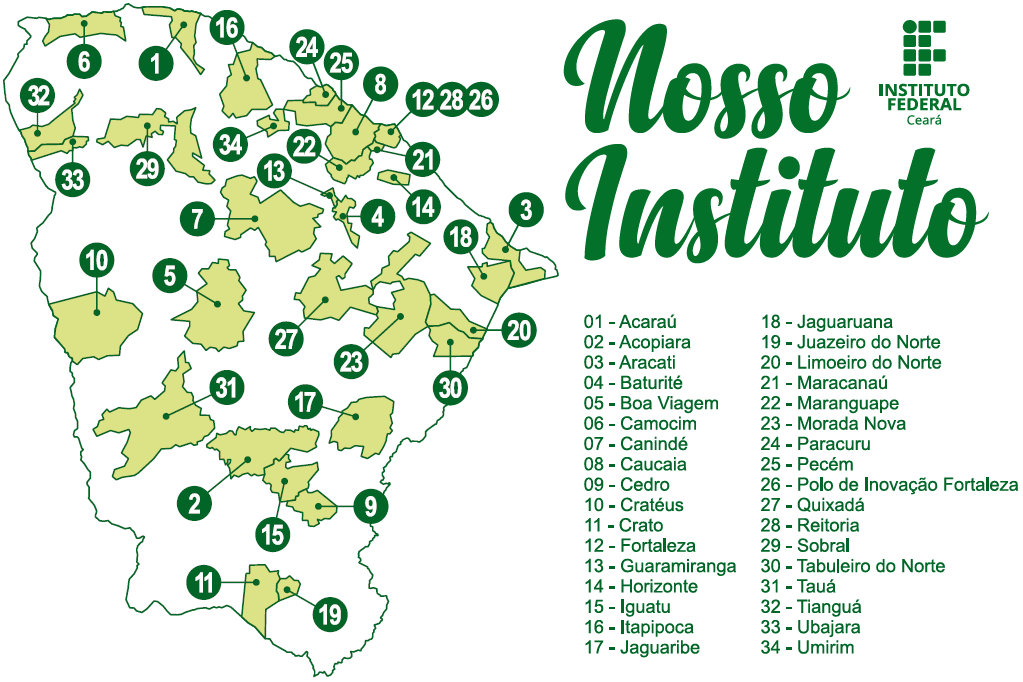
\includegraphics[scale=0.5]{figuras/ifce-estado}
\Fonte{Instituto Federal de Educação, Ciência e Tecnologia do Ceará (2018).}
\end{figure}

\newpage

\subsubsubsection{Título da seção quinária}

As tabelas - apresentação de informações, de forma não discursiva, nas quais o dado numérico se destaca como informação central - devem ser inseridas o mais próximo possível do texto a que se referem.

Sua identificação aparece na parte superior, composta pelo nome tabela, seguido do número de ordem de ocorrência no texto, em algarismos arábicos, travessão e do respectivo título, ajustados às margens da tabela, em espaço simples (1,0) e alinhamento justificado.

\begin{table}[!ht]	
\Caption{Estimativas populacionais brasileiras - Regiões - 2011-2017}
\centering
\label{estimativas}
\begin{tabular}{c|c|c|c|c|c}
\hline
& \multicolumn{5}{c}{\textbf{Regiões}} \\
\cline{2-6}
\textbf{Ano} & \textbf{Sudeste} & \textbf{Nordeste} & \textbf{Sul} & \textbf{Norte} & \textbf{Centro-Oeste} \\
\hline
2011 & 80.975.616 & 53.501.859 & 27.562.433 & 16.095.187 & 14.244.192 \\
\hline
2012 & 81.565.983 & 53.907.144 & 27.708.514 & 16.303.145 &
14.419.229 \\
\hline
2013 & 84.465.570 & 55.794.707 & 28.795.762 & 16.983.484 &
14.993.191 \\
\hline
2014 & 85.115.623 & 56.186.190 & 29.016.114 & 17.231.027 &
15.219.608 \\
\hline
2015 & 85.745.520 & 56.559.481 & 29.230.180 & 17.472.636 &
15.442.232 \\
\hline
2016 & 86.356.952 & 56.915.936 & 29.439.773 & 17.707.783 &
15.660.988 \\
\hline
2017 & 86.949.714 & 57.254.159 & 29.644.948 & 17.936.201 &
15.875.907 \\
\hline
\end{tabular}
\Fonte{Instituto Brasileiro de Geografia e Estatística (2018).}
\end{table}

\begin{flushright}
\begin{minipage}[b]{13.9cm}
\begin{SingleSpace}
\begin{footnotesize}
Notas: Em 2012: \\
\hspace*{0.9cm}
1 - Por determinação judicial e para efeito de distribuição do Fundo de Participação dos Municípios, a população do Município de Brasil Novo-PA é de 17.960 habitantes. Processo Judicial nº 1-28.2012.4.01.3903. \\
\hspace*{0.9cm} 2 - Por determinação judicial e para efeito de distribuição do Fundo de Participação dos Municípios, a população do Município de Jacareacanga-PA é de 41.487 habitantes. Processo Judicial nº 798-41.2011.4.01.3902, Seção Judiciária de Itaituba-PA. \\
\hspace*{0.9cm} Em 2013: \\
\hspace*{0.9cm} Por determinação judicial e para efeito de distribuição do Fundo de Participação dos Municípios, a população do Município de Jacareacanga-PA é de 41.487 habitantes. Processo Judicial nº 798-41.2011 4.01.3902 Seção Judiciária de Itaituba-PA. \\
\hspace*{0.9cm} Em 2014: \\
\hspace*{0.9cm}1 - Por determinação judicial e para efeito de distribuição do Fundo de Participação dos Municípios, a população do Município de Jacareacanga-PA é de 41.487 habitantes. Processo Judicial nº 798-41.2011.4.01.3902, Seção Judiciária de Itaituba-PA. \\
\hspace*{0.9cm} 2 - Por determinação judicial o Município de Coronel João Sá - BA teve os efeitos das estimativas das populações de 2014, 2015 e 2016 suspensas, passando a vigorar, para efeito de distribuição do Fundo de Participação dos Municípios, a população estimada para o ano de 2013, que foi de 17.422 habitantes. Processo Judicial nº 0002222-53.2017.4.01.3306 - Vara Única de Paulo Afonso-BA.
\end{footnotesize}
\end{SingleSpace}
\end{minipage}
\end{flushright}

\newpage

Além do número da população residente, foram extraídas do Portal do IBGE informações populacionais com as variáveis apresentadas no quadro a seguir.

A identificação do quadro aparece na parte superior, composta por seu nome, seguido do número de ordem de ocorrência no texto, em algarismos arábicos, travessão e do respectivo título, ajustados às margens do quadro, em espaço simples (1,0) e alinhamento justificado\footnote{As notas de rodapé têm por finalidade prestar esclarecimentos ou fazer considerações sobre certos aspectos que não devem ser incluídos no texto para não interromper a sequência lógica da leitura.}.

\begin{quadro}[!ht]	
\Caption{Características da população brasileira pesquisadas}
\centering
\label{qua:exemplo-1}
\IFCEqua{}{
\begin{tabular}{|l|l|}
\hline
\textbf{Tema} & \textbf{Variáveis} \\
\hline
Características gerais da população & População residente, situação de domicílio, sexo e idade \\
\hline
Cor ou raça & População residente, idade, sexo, situação de domicílio, educação \\
\hline
Educação & Taxa de alfabetização \\
\hline
Emigração & Emigrantes internacionais \\
\hline
Registro de nascimento & Idade, situação de domicílio, sexo, cor ou raça \\
\hline
Trabalho e rendimento & Idade, sexo, cor ou raça, Índice de Gini \\
\hline
\end{tabular}
}{
\Fonte{Instituto Brasileiro de Geografia e Estatística (2010).}
}
\end{quadro}

\newpage

Para acompanhar o crescimento populacional\footnote{As notas devem constar na mesma página em que ocorre a chamada numérica no texto, digitadas com espaçamento simples (1,0) entre as linhas e alinhadas, a partir da segunda linha da mesma nota, abaixo da primeira letra da primeira palavra, de forma a destacar o expoente, sem espaço entre elas e com fonte tamanho 10.}, anualmente, o IBGE publica estimativas populacionais do nosso país, com dados das regiões, dos estados e, até, dos 5.570 municípios brasileiros\footnote{As notas podem ser de dois tipos: notas de referência e notas explicativas, conforme o Manual de Normalização de Trabalhos Acadêmicos do IFCE.}. 
% \input{elementos-textuais/trabalhos-relacionados}
% % \chapter{Título da Seção Primária}

% \begin{figure}[!h]
%     \centering
%     \Caption{\label{fig:exemplo-2}Exemplo de Figura}
%     \IFCEfig{}{
%         \fbox{
\includegraphics[width=8cm]{figuras/logo-ifce}}
%     }{
%         \Fonte{Elaborado pelo autor}
%     }
% \end{figure}

% \begin{table}[!h]
%     \centering
%     \Caption{\label{tab:exemplo-2} Exemplo de Tabela}
%     \IFCEtab{}{
%         \begin{tabular}{cll}
%             \toprule
%             Texto             & Texto             & Texto             \\
%             \midrule \midrule
%             Texto texto texto & Texto texto texto & Texto texto texto \\
%             Texto texto texto & Texto texto texto & Texto texto texto \\
%             Texto texto texto & Texto texto texto & Texto texto texto \\
%             Texto texto texto & Texto texto texto & Texto texto texto \\
%             Texto texto texto & Texto texto texto & Texto texto texto \\
%             Texto texto texto & Texto texto texto & Texto texto texto \\
%             \bottomrule
%         \end{tabular}
%     }{
%         \Fonte{Elaborado pelo autor}
%     }
% \end{table}

% \begin{quadro}[!h]
%     \centering
%     \Caption{\label{qua:exemplo-3} Exemplo de Quadro}
%     \IFCEqua{}{
%         \begin{tabular}{|c|c|l|l|}
%             \hline
%             Texto             & Texto             & Texto             & Texto             \\
%             \hline
%             Texto texto texto & Texto texto texto & Texto texto texto & Texto texto texto \\
%             \hline
%             Texto texto texto & Texto texto texto & Texto texto texto & Texto texto texto \\
%             \hline
%             Texto texto texto & Texto texto texto & Texto texto texto & Texto texto texto \\
%             \hline
%         \end{tabular}
%     }{
%         \Fonte{Elaborado pelo autor}
%     }
% \end{quadro}

% \newpage

% \begin{center}
%     Exemplo de referência \\
%     Livro: \cite{knuth} \\ Dissertação: \cite{Maia2011} \\ Artigo: \cite{lamport1986latex}
% \end{center}

% \begin{center}
%     Exemplo de Alíneas com Número
% \end{center}
% \begin{alineascomnumero}
%     \item Texto texto texto.
%     \item Texto texto texto.
%     \item Texto texto texto.
%     \item Texto texto texto.
%     \item Texto texto texto.
% \end{alineascomnumero}

% \begin{center}
%     Exemplo de Alíneas com Ponto
% \end{center}
% \begin{alineascomponto}
%     \item Texto texto texto.
%     \item Texto texto texto.
%     \item Texto texto texto.
%     \begin{subalineascomponto}
%         \item Texto texto texto.
%         \item Texto texto texto.
%     \end{subalineascomponto}
% \end{alineascomponto}
\chapter{Metodologia}
Com base em Marconi e Lakatos (2001), como estaremos utilizando métodos matemáticos, lógicos e estatísticos para esta pesquisa,
determinamos que esta terá caráter quantitativo.

Para esta pesquisa, estaremos utilizando os motores de xadrez chamados \textit{Stockfish}, \textit{Leela Chess Zero} (LCZ),
\textit{RubiChess}, \textit{Nemorino}, \textit{Igel}, \textit{Xifos}, \textit{Laser}, \textit{Defenchess}, \textit{Andscacs},
\textit{Halogênio}, \textit{Arasan} e o \textit{Combusken}, todos de código aberto.

A comparação que faremos entre os motores vai ser pela sua velocidade em calcular as melhores jogadas, a qualidade de movimentos,
sua porcentagem de vitórias e por seu ranking nos campeonatos de motores online, sendo o mais famoso deles o \textit{Top Chess Engine Championship}.

Primeiro começaremos avaliando a implementação da representação do tabuleiro de cada um dos motores de xadrez selecionados,
descrevendo como é a estrutura de dados que guarda: as posições de todas as peças, a informação de qual dos jogadores
é a vez, o direito de \textit{roque}, a casa com possibilidades de captura \textit{en passant} e o número de movimentos relacionado
a regra de 50 movimentos. Também mediremos quão boa a representação do tabuleiro com base nas três principais
formas de representação: centrada nas peças, centrada nas casas e a híbrida.


Depois de analisarmos a base do motor, iremos calcular a velocidade mínima, média e de pior caso de cada um dos algoritmos
apontados neste trabalho, levando em conta as variáveis de quantidade de peças em jogo, possíveis movimentos de \textit{roque}
e captura \textit{en passant}. Além de a partir das referências já citadas e seus diferentes métodos de cálculo de avaliação
de movimentos, verificar quais dos algoritmos produzem os melhores movimentos.

Criaremos uma estrutura de teste para verificar a porcentagem de vitórias de cada motor de xadrez, investigando
a participação de cada algoritmo nesta porcentagem. Levaremos em conta o elo ou \textit{ranking} dos motores em campeonatos,
seus feitos já realizados, e possíveis erros e \textit{bugs} encontrados.

Por fim, analisaremos quais possíveis mudanças e efeitos diferentes algoritmos de comunicação entre dois motores
e uma interface podem produzir dentro dos fatores aos quais iremos comparar os motores.

% \input{elementos-textuais/resultados}
% \chapter{Conclusão}

É a parte que sintetiza os argumentos e elementos contidos no desenvolvimento do trabalho, em que são apresentadas as conclusões próprias da pesquisa, retomando o problema inicial e os objetivos e revendo as principais contribuições do estudo (\cite{andrade}; \cite{koche}; \cite{barros}).

O título dessa parte será \textbf{CONCLUSÃO} quando o conteúdo desenvolvido no trabalho permitir resultados conclusivos. No caso de pesquisas não conclusivas, pode-se intitular essa seção como \textbf{CONSIDERAÇÕES FINAIS} \cite{andrade}.

% Elementos pós-textuais

\imprimirreferencias{elementos-pos-textuais/referencias}
%\imprimirglossario	
\imprimirapendices
% \apendice{Relação de Normas Técnicas vigentes utilizadas na Normalização de Trabalhos Científicos}

\begin{quadro}[!ht]	
\centering
\Caption{\label{qua:exemplo-2} Normas técnicas vigentes sobre normalização de trabalhos acadêmicos do ABNT/CB - 014}
\IFCEqua{}{
\begin{tabular}{|c|c|}
\hline
\textbf{Número} & \textbf{Título} \\
\hline
6022:2018 & Artigo em publicação periódica técnica e/ou científica - Apresentação \\
\hline
6023:2002 & Referências - Elaboração \\
\hline
6024:2012 & Numeração progressiva das seções de um documento - Apresentação \\
\hline
6027:2012 & Sumário - Apresentação \\
\hline
6028:2003 & Resumo - Apresentação \\
\hline
6034:2004 & Índice - Apresentação \\
\hline
10520:2002 & Citações em documentos - Apresentação \\
\hline
10719:2015 & Relatório técnico e/ou científico - Apresentação \\
\hline
12225:2004 & Lombada - Apresentação \\
\hline
14724:2011 & Trabalhos acadêmicos - Apresentação \\
\hline
15287:2011 & Projeto de pesquisa - Apresentação \\
\hline
15437:2006 & Pôsteres técnicos e científicos - Apresentação \\
\hline
\end{tabular}
}{
\Fonte{elaborado pelo autor, de acordo com o Catálogo da ABNT.}
}
\end{quadro}
\imprimiranexos
% \anexo{Resolução que aprova a criação do Curso Superior de Tecnologia em Gestão Ambiental no IFCE \textit{Campus} Paracuru}

\begin{center}
\begin{figure}[!ht]
\centering
%\Caption{\label{fig:exemplo-2}xxx}	
\IFCEfig{}{
\fbox{
\includegraphics[width=2.5cm]{figuras/brasao-brasil}}
}{
%\Fonte{xxx}
}	
\end{figure}
\vspace*{-0.8cm}
\textbf{
SERVIÇO PÚBLICO FEDERAL \\
INSTITUTO FEDERAL DE EDUCAÇÃO, CIÊNCIA E TECNOLOGIA DO CEARÁ \\
CONSELHO SUPERIOR
}
\end{center}

\begin{center}
\textbf{RESOLUÇÃO N° 01, DE 10 DE JANEIRO DE 2018}
\end{center}

\vspace*{-1cm}

\begin{SingleSpace}
\begin{flushright}
\begin{minipage}[b]{8cm}
\begin{small}
Aprova \textit{ad referendum} a criação do curso Superior de Tecnologia em Gestão Ambiental no \textit{campus} Paracuru. 
\end{small}
\end{minipage}
\end{flushright}
\end{SingleSpace}

\textbf{O PRESIDENTE EM EXERCÍCIO DO CONSELHO SUPERIOR DO INSTITUTO FEDERAL DE EDUCAÇÃO, CIÊNCIA E TECNOLOGIA DO CEARÁ}, no uso de suas atribuições legais e estatutárias e considerando o Memorando n$^{\circ}$ 001/2018/GDG da direção-geral do campus Paracuru, 

\textbf{RESOLVE:}

\textbf{Art. $1^{\circ}$} - Criar, \textit{ad referendum} do Conselho Superior, o curso Superior de Tecnologia em Gestão Ambiental do \textit{campus} Paracuru e autorizar a oferta de 35 vagas semestrais.

\textbf{Parágrafo único} - O curso será ofertado na modalidade presencial e nos turnos matutino e vespertino, conforme definido no projeto pedagógico em anexo. 

\textbf{Art. $2^{\circ}$} - A interrupção da oferta e/ou a extinção do referido curso deverá ser submetida a este conselho para aprovação, com as devidas justificativas e a apresentação do planejamento de realocação de recursos humanos e de materiais vinculados ao curso.

\begin{center}
José Wally Mendonça Menezes \\
\textbf{Presidente em exercício do Conselho Superior}
\end{center}
%\imprimirindice

\end{document}